\chapter{Experimentation}
\label{ch_experimentation}
%This is a chapter added into the template because Dr. Winberg's example reports have it.

\section{Testing Methodology}

Testing was performed in two phases, the first phase involves testing of individual modules. This modular testing is analogous to unit-tests in the computer programming paradigm. The second phase of testing involves characterising the performance of the final system prototype.

\subsection{Focal Length of Lens}
\label{exp:focal_length}
To generate the beam of light from the IR LED, a light focusing tube was created with a lens as described in the design section. To determine the dimensions of the light focusing tube, the focal length of the lens needed to be measured.

Figure \ref{fig:focal_length_experiemnt} shows the experimental setup used to determine the focal length of the lens. The lens was secured to a pair of 'helping-hands' to allow for precise adjustment of height above the working surface. A light source was placed directly above the lens at a distance of 1.2m.

\begin{figure}[H]
		\centering
		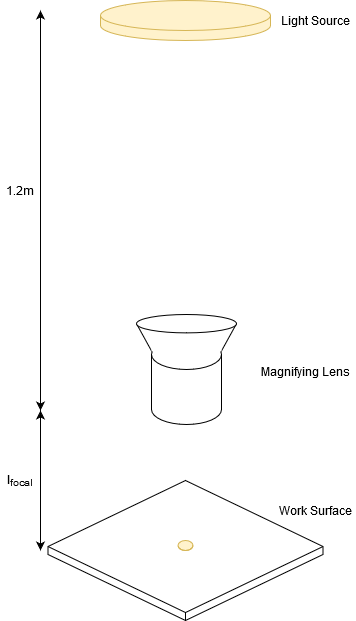
\includegraphics[width=.4\linewidth]{figures/experimentation/focal_length.png}
		\captionof{figure}{Focal Length Experiment Setup}
		\label{fig:focal_length_experiemnt}
\end{figure}

After setting up the experiment, the lens was slowly adjusted along the vertical until the spot formed on the work surface was a minimum. A tape measure was used to find the distance from the work surface to the lens.

\subsection{Light Focus System}

To test the light focusing tube, two power LEDs where used. Initially, a 3W warm white (visible light) power LED was used to confirm the functionality of the system. Following this, the 3W IR power LED was used.

In both cases, the focus system was setup a specific distance from a flat surface. The light was then powered and the edge of the beam spot was marked and the diameter taken. To determine the location of the IR beam spot edge, a video camera in 'night shot' mode was used.

\begin{figure}[H]
	\centering
	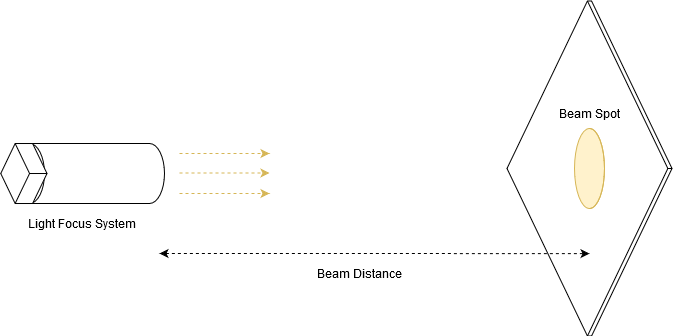
\includegraphics[width=.7\linewidth]{figures/experimentation/beam_spot_experiement.png}
	\captionof{figure}{Light Focus System Experiment Setup}
	\label{fig:focus_system_experiemnt}
\end{figure}

%todo: Give distances for measuredments taken
Figure \ref{fig:focus_system_experiemnt} above shows the experimental setup. The experiment was performed for distances of x, y, z.
















\newpage
\subsection{Tests $\setminus$ Results to gather}
\textbf{Hardware}
\begin{itemize}
	\item IR Power LED:
	\begin{itemize}
		\item Beam angle (focus vs no focus)
		\item Beam strength (LUX)
		\item LED Current draw
		\item LED temperature (basic sensor or a temperature gun that I borrow from somewhere)
		\item MOSFET temperature
	\end{itemize}
	\item For each photo-sensor (photodiode, phototransistor, all in one receiver module):
	\begin{itemize}
		\item Receiving beam-angle
		\item Output signal strength vs light-intensity/distance
		\item Reaction time (rise time)
		\item multipath/picking up reflections
		\item Signal to noise ration
	\end{itemize}
	\item Op-Amp:
	\begin{itemize}
		\item Op-amp gain performance (push to limit) (at 36kHz)
		\item Op-amp frequency performance (at some fixed gain)
		\item Filter performance (anti-aliasing and high pass filtering)
	\end{itemize}
\end{itemize}

\textbf{Software}
\begin{itemize}
	
	\item Transmitter
	\begin{itemize}
		\item Timing accuracy
	\end{itemize}
	
	%\item Protocol
	%\begin{itemize}
	%	\item
	%\end{itemize}
	
	\item Receiver
	\begin{itemize}
		\item Bit error rate / max receiver distance - (not sure how I will implement this yet)
		\item Bit error correction - (not sure how I might implement this yet)
		\item Modulation to High/Low logic value [DSP processing analysis]
		\begin{itemize}
			\item Latency
			\item Testing the timing between stages of demodulating and decoding
		\end{itemize}
	\end{itemize}
	
\end{itemize}